% !TEX root = ../main.tex
% Many real-world applications of probability theory have one particular feature that data are collected sequentially in time.
% A few examples are weather data, stock market indices, air-pollution data, demographic data, and political tracking polls.
% These also have antoher feature in common that successive observations are typically not independent.
% We refer to any such collection of abservation as a \textit{stochastic process}.
% Formally, a stochastic process is a collection of random variables that take values in a set $S$, the \textit{state space}.
% The collection is indexed by another set $T$ the \textit{index set}.
% The two most common sets are the natural numbers $T = \{0, 1, 2, \ldots\}$ and the non negative real numbers $T = [0, \infty)$, which usually represent discrete time and continuous time, respectively.
% The first index set thus gives a sequence of random variables $\{X_0, X_1, X_2, \ldots \}$ and the second, a  collection of random variables $\{X(t), t \geq 0 \}$, one random variable for each time $t$.
% In general, the index set does not have to describe time and is also commenly use to describe spatial location.
% The state space can be finite, countably infinite, or uncountable, depending on the application.

\subsection{Discrete-Time Markov Chains}
\begin{boks}{Definition 8.1.}
  Let $X_0, X_1, X_2, \ldots$ be a sequence of discrete random variables, taking values in some set $S$ and that are such that
  \begin{align}\label{eq:markov_egenskaben}
    P(X_{n + 1} = j | X_0 = i_0, \ldots, X_{n - 1} = i_{n - 1}, X_n = i) =
    P(X_{n + 1} = j | X_n = i)
  \end{align}
  for all $i, j, i_0, \ldots, i_{n - 1}$ in $S$ and all $n$. The sequence $\{ X_n \}$ is then called a \textit{Markov chain}. Furthermore \eqref{eq:markov_egenskaben} is called the \textit{Markov property}.
\end{boks}
We ofthen think of the index $n$ as discrete time and say that $X_n$ is the \textit{state} of the chain at time $n$, where the state space $S$ may be finite or coutably infinte.

% In general, the probability $P(X_{n + 1} = j | X_n = i)$ depends in $i,j$, and $n$. It is, however, often the case that there is no dependence on $n$. We call such chains \textit{time-homogenous} and restrict our attention to these chains. Since the conditional probability in the definition thus depends only on $i$ and $j$, we use the notation
\begin{align*}
  p_{ij} = P(X_{n + 1} = j | X_n = i), \quad i,j \in S
\end{align*}
% and call these the \textit{transition probabilities} of the Markov chain. Thus, if the chain is in state \textit{i}, the probabilities $p_{ij}$ desribe how the chain chooses which state to jump to necxt. Obviously, the transition probabilities have to satisfy the following two criteria:
\begin{align*}
  \text{(a)} \ p_{ij} \geq 0 \quad \text{for all} \ i,j \in S, \qquad
  \text{(b)} \ \sum_{j \in S} p_{ij} = 1 \quad \text{for all} \ i \in S
\end{align*}

\begin{figure}[h]
  \centering
  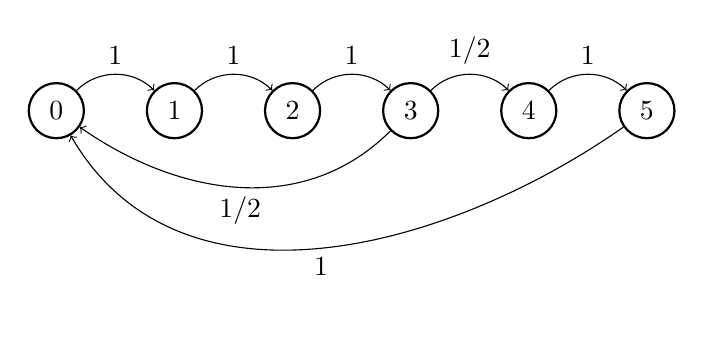
\begin{tikzpicture}[roundnode/.style={circle, draw=black, thick, minimum size=7mm}]
    % Place nodes
    \node[roundnode] (nul)                                        {0};
    \node[roundnode] (et)   [right of = nul, node distance=15mm]  {1};
    \node[roundnode] (to)   [right of = et, node distance=15mm]   {2};
    \node[roundnode] (tre)  [right of = to, node distance=15mm]   {3};
    \node[roundnode] (fire) [right of = tre, node distance=15mm]  {4};
    \node[roundnode] (fem)  [right of = fire, node distance=15mm] {5};
    % Create edges
    % Above
      \draw[->] (nul)   to [out = 45, in = 135] node[above] {1}   (et);
      \draw[->] (et)    to [out = 45, in = 135] node[above] {1}   (to);
      \draw[->] (to)    to [out = 45, in = 135] node[above] {1}   (tre);
      \draw[->] (tre)   to [out = 45, in = 135] node[above] {1/2} (fire);
      \draw[->] (fire)  to [out = 45, in = 135] node[above] {1}   (fem);
    % Below
      \draw[->] (tre) to [out = 225, in = 325] node [below] {1/2} (nul);
      \draw[->] (fem) to [out = 215, in = 300] node [below] {1}   (nul);
  \end{tikzpicture}
\end{figure}

% \subsubsection{Time Dynamics of a Markov Chain}
% The most fundamental aspect of a Markov chain in which we are interested is how it develops over time.
% The transition matrix provides us with a despriction od the stepwise behaviour, but suppose that we want to compute the distribution of the chain two steps ahead. Let
% \begin{align*}
%   p_{ij}^{(2)} = P(X_2 = j | X_0 = i)
% \end{align*}
% and condition on the intermediate step $X_1$. The law of total probability gives
% \begin{align*}
%   p_{ij}^{(2)} &= \sum_{k \in S} P(X_2 = j | X_0 = i, X_1 = k)
%   P(X_1 = k | X_0 = i) \\
%   &=\sum_{k \in S} P(X_2 = j | X_1 = k) P(X_1 = k | X_0 = i) =
%   \sum_{k \in S} p_{ik}p_{kj}
% \end{align*}
% where we used the Markov property for the second-to-last equality. We switched the order between the factors in the sum to get the intuitively appealing last expression; in order to fo from $i$ to $j$ in two steps, we need to visit intermediate step $k$ and jump from there to $j$. Now, recall how matrix multiplication works to help us realize from the expression above that $p_{ij}^{(2)}$ is the $(i, j)$th entry in the matrix $P^2$. Thus, in order to get the two-step transition probabilities, we square the transition matrix. Generally, define the \textit{n-step transition probabilities} as
% \begin{align*}
%   p_{ij}^{(n)} = P(X_n = j | X_0 = i)
% \end{align*}
% and let $P^{(n)}$ be the $n$-step transition matrix. Repeating the argument above gives $P^{(n)} = P^n$, the $n$th power of the one-step transition matrix. In particular, this gives the relation
% \begin{align*}
%   P^{(n + m)} = P^{(n)}P^{(m)}
% \end{align*}
% for all $m, n$, commonly referred to as the \textit{Chapman-Kolmogorov equations}. Spelld out coordinatewise, they become
% \begin{align*}
%   p_{ij}^{(n + m)} =  \sum_{k \in S} p_{ik}^{(n)}p_{jk}^{(m)}
% \end{align*}
% for all $m, n$ and all $i,j \in S$. In words, to go from $i$ to $j$ in $n + m$ steps, we nedd to visit some intermediate step $k$ after $n$ steps. We let $P^{(0)} = I$, the identity matrix.

\subsubsection{Classification of States}
\begin{boks}{Definition 8.2}
  If $p_{ij}^{(n)} > 0$ for some $n$, we say that state $j$ is \textit{accesible} from state $i$, written $i \rightarrow j$. If $j \rightarrow i$, we say that $i$ and $j$ \textit{communicate} and write this $i \leftrightarrow j$.
\end{boks}
% In general, if we fix a state $i$ in the state space of a Mrkov vhain, we can find all states that communicate with $i$ and form a \textit{communicating class} containing $i$. It is easy to realize that not only does $i$ communicate with all states in this class but they all communicate with each other. By convention, every state communicates with itself (it can reach itself in $0$ steps) so every state belongs to a class.
% If you wish to be more mathemaical, the relastion ``$\leftrightarrow$'' is an equivalence relation and thus divides the state space into equivalence classes that are precisely the communicating classes.
\begin{boks}{Definition 8.3}
  If all states in $S$ communicate with each other, the Markov chain is said to be \textit{irreducible}.
\end{boks}
This means that our Markov chain we are is irreducible.
\begin{boks}{Definition 8.4}
  Consider a state $i \in S$ and the $\tau_i$ be the number of steps it takes for the chain to first visit $i$. Thus
  \begin{align*}
    \tau_i = \min \{ n \geq 1 \ : \ X_n = i \}
  \end{align*}
  where $\tau_i = \infty$ if $i$ is never visited. If $P_i(\tau_i < \infty) = 1$, the state $i$ is said to be \textit{recurrent} and if $P_i(\tau_i < \infty) < 1$, it is said to be \textit{transient}.
\end{boks}
We can conclude that all states in our chain is recurrent.
% \begin{boks}{Corollary 8.1}
%   In an irreducible Markov chain, either all states are trasient or all states are recurrent.
% \end{boks}
% \begin{boks}{Corollary 8.2}
%   Suppose that $S$ is finite. A state $i$ is transient if and only if there is another state $j$ such that $i \rightarrow j$ but $j \nrightarrow i$.
% \end{boks}
% \begin{boks}{Corollary 8.3}
%   If a Markov chain has finite state space, there is at least one recurrent state.
% \end{boks}
% \begin{boks}{Proposition 8.1}
%   State $i$ is
%   \begin{align*}
%     \text{transient if} \quad &\sum_{n = 1}^\infty p_{ii}^{(n)} < \infty \\
%     \text{recurrent if} \quad &\sum_{n = 1}^\infty p_{ii}^{(n)} = \infty
%   \end{align*}
% \end{boks}

\subsubsection{Stationary Distribution}
\begin{boks}{Definition 8.5}
  Let $P$ be the transition matrix of a Markov chain with state space $S$. A probability distribution $\boldsymbol{\pi} = (\pi_1, \pi_2, \ldots)$ on $S$ satisfying
  \begin{align*}
    \boldsymbol{\pi} P = \boldsymbol{\pi}
  \end{align*}
  is called a \textit{stationary distribution} of the chain.
\end{boks}
\begin{boks}{Proposition 8.2}
  Consider an irreducible Markov chain. If a stationary distribution exists, it is unique.
\end{boks}
\begin{boks}{Proposition 8.3}
  If $S$ is finite and the Markov chain is irreducible, a unique stationary distribution $\boldsymbol{\pi}$ exists.
\end{boks}
The transition matrix for our chain in given as the following
\begin{align*}
  P =
  \begin{bmatrix}
      0 & 1 & 0 & 0 & 0 & 0  \\
        &   & 1 &   &     &  \\
        &   &   & 1 &     &  \\
    1/2 &   &   &   & 1/2 &  \\
        &   &   &   &     &1 \\
    1   &   &   &   &     &
  \end{bmatrix}
\end{align*}
The stationary distribution is defined at
\begin{align*}
  \pi P = \pi
\end{align*}
From Proposition 8.3 we can conclude that a unique stationary distribution exists
\begin{align*}
  \pi_0 = \frac{1}{2} + \pi_5, \quad
  \pi_1 = \pi_0, \quad
  \pi_2 = \pi_1, \quad
  \pi_3 = \pi_2, \quad
  \pi_4 = \frac{1}{2} \pi_3, \quad
  \pi_5 = \pi_4
\end{align*}
This gives the stationary distribution
\begin{align*}
  \pi = \left[\frac{1}{5}, \frac{1}{5}, \frac{1}{5}, \frac{1}{5}, \frac{1}{10}, \frac{1}{10}\right]
\end{align*}
\begin{boks}{Definition 8.6}
  Let $i$ be a recurrent state. If $E_i[\tau_i] < \infty$, then $i$ is said to be \textit{positive recurrent}. If $E_i[\tau_i] = \infty$, $i$ is said to be \textit{null recurrent}.
\end{boks}
\begin{boks}{Corollary 8.4}
  For an irreducible Markov chain, there are three possibilities: \textbf{(a)} all states are positive recurrent, \textbf{(b)} all states are null recurrent, and \textbf{(c)} all states are transient.
\end{boks}
% \begin{boks}{Proposition 8.4}
%   Consider an irreducible Markov chain $\{ X_n \}$. Then,
%   \begin{align*}
%     \text{A stationary distribution} \ \boldsymbol{\pi} \ \text{exists} \Leftrightarrow \{ X_n \} \ \text{is positive recurrent}
%   \end{align*}
%   If this is the case, $\boldsymbol{\pi}$ is unique and has $\pi_j > 0$ for all $j \in S$.
% \end{boks}

\begin{boks}{Definition 8.8}
  The \textit{period} of state $i$ is defined as
  \begin{align*}
    d(i) = \gcd \{ n \geq 1 \ : \ p_{ii}^{(n)} > 0 \}
  \end{align*}
  the greatest common divisor of lengths of cycles through which it is possible to return to $i$. If $d(i) = 1$, state $i$ is said to be \textit{aperiodic}; otherwise it is called \textit{periodic}. Note that this is a class property, which means if $i \leftrightarrow j$ and either $i$ or $j$ is periodic so is the other. Likewise for aperiodic.
\end{boks}

In our chain we observe that a state can reach itself in either $4$ or $6$ steps, which means that all states in our chain is periodic with period $2$, because this is the greatest common divisor of $4$ and $6$.
% \subsubsection{Convergence to the Stationary Distribution}
% \begin{boks}{Definition 8.7}
%   Let $p_{ij}^{(n)}$ be the $n$-step transition probabilities of a Markov chain.
%   If there exists a probability distribution \textbf{q} on $S$ such that
%   \begin{align*}
%     p_{ij}^{(n)} \rightarrow q_j \quad \text{as} \quad n \rightarrow \infty \quad \text{for all} i,j \in S
%   \end{align*}
%   we call \textbf{q} the \textit{limit distribution} of the Markov chain.
% \end{boks}
% \begin{boks}{Theorem 8.1}
%   Consider an irreducible, positive recurrent, and aperiodic Markov chain with stationary distribution $\boldsymbol{\pi}$ and $n$-step transition probabilities $p_{ij}^{(n)}$. Then
%   \begin{align*}
%     p_{ij}^{(n)} \rightarrow \pi_j \quad \text{as} \quad n \rightarrow \infty
%   \end{align*}
%   for all $i,j \in S$.
% \end{boks}
% An irreducible, positve recurrent, and aperiodic Markov chain is called \textit{ergodic}.
% \begin{boks}{Proposition 8.5}
%   Consider an ergodic Markov chain with stationary distrbution $\boldsymbol{\pi}$ and choose two states $i$ and $j$. Let $\tau_i$ be the return tome to state $i$, and let $N_j$ be the number of visits to $j$ between consecutive visits to $i$. Then
%   \begin{align*}
%     E_i[\tau_i] = \frac{1}{\pi_i} \quad \text{and} \quad
%     E_i[N_j] = \frac{\pi_j}{\pi_i}
%   \end{align*}
% \end{boks}
% Note that by positive recurrence, all the $E_i[\tau_i]$ are finite and hence all the $\pi_i$ are strictly positive. The $E_i[\tau_i]$ are called the \textit{mean recurrence times}.
